\documentclass[10pt,a4paper]{article}
\usepackage[margin=20mm]{geometry}
\usepackage[T1]{fontenc}
\usepackage{lmodern,microtype,amsmath,amssymb,booktabs,tabularx,array,graphicx}
\usepackage{float}
\usepackage[hidelinks]{hyperref}
\setlength{\parindent}{0pt}\setlength{\parskip}{5pt}
\graphicspath{{generated/}}
\begin{document}
\begin{center}
{\LARGE\bfseries Learning When to Search for\\[3pt] Multi Agent Path Finding}\par
\vspace{5pt}{\large A gated hybrid of learned policies and heuristic search}\par
\vspace{8pt}\textbf{Abhivansh Gupta (23112004)\quad Shivang Joshi (23117132)}\\
IIT Roorkee\quad |\quad Project Report\quad |\quad November 2026
\end{center}
\begin{abstract}
Local learned policies select actions quickly but can produce persistent coordination failures. We implement a hybrid of a shielded imitation policy, policy-guided priority inheritance with backtracking (CS-PIBT), and a budgeted LaCAM fallback. A logistic gate uses sixteen features and labels from eight-step search-versus-policy rollouts. On 140 unseen random-grid instances with 16--192 agents, the hybrid solves all tested instances while using approximately 23--57\% fewer external CS-PIBT calls than always-search. At 192 agents, its common-subset flowtime ratio is 1.601, versus 2.286 for random gating with fallback. However, without fallback, random triggering is stronger across much of the observed rate range. Plain LaCAM is also faster on these maps. The results demonstrate selective coordination and its limitations, rather than a new optimal solver or a general speed advantage.
\end{abstract}
\section{Introduction and objectives}
Multi-agent path finding (MAPF) coordinates agents travelling from individual starts to goals in a shared environment. Individually short routes may conflict when executed simultaneously. A local learned policy proposes moves in one batched network call, while heuristic search explicitly coordinates the team. Our question is whether we can learn \emph{when} to use search instead of invoking it at every step.

The project implements the environment, imitation policy, collision shield, PIBT, policy-guided CS-PIBT, LaCAM and a logistic search gate. We compare task completion, solution quality, search invocations and runtime, and provide a visual replay. The idea was jointly developed by the members; implementation, analysis and documentation were prepared with AI assistance. The separate contribution statement records shared ideation and assigned review responsibilities.

\subsection{Related work}
Veerapaneni et al.~\cite{veerapaneni} combine local learned MAPF policies with heuristic search, motivating policy-guided coordination. PIBT~\cite{pibt} provides recursive priority inheritance and backtracking. LaCAM~\cite{lacam} searches joint configurations using lazy constraints. Phan et al.~\cite{address} direct anytime MAPF optimisation toward useful agent neighbourhoods with ADDRESS. That work motivates selective computational effort, but ADDRESS and large-neighbourhood search are not implemented here. Our gate chooses when the whole team uses one-step search.

\section{Problem formulation}
The map is a four-connected graph $G=(V,E)$ with static obstacles. Agent $i$ starts at $s_i$, targets $g_i$ and can wait or move one free cell in a cardinal direction. The joint configuration is $Q_t=(v_1^t,\ldots,v_N^t)$. Valid motion forbids two agents occupying the same cell and forbids exchanging cells in one step.

We measure flowtime $J(P)=\sum_i T_i$ and makespan $M(P)=\max_i T_i$. Agents may leave goals to coordinate, so $T_i$ is final arrival after which the agent remains at its goal through the end of the plan. BFS computes static shortest distances $d_i(v)$ ignoring other agents. The lower bound $L=\sum_i d_i(s_i)$ gives quality ratio $J/L$ for completed solutions. It is not a ratio to a known optimal joint plan. Safe movement and eventual completion are separate properties.

\newpage
\section{Method}
\subsection{Policy and collision shield}
The map is $32\times32$ cells. Each agent receives four channels on an $11\times11$ window: obstacles, other agents, relative cost-to-go and its goal if visible. The radius of five is a design choice, not an established optimum. The distance channel comes from the full static map, so the local crop still contains map-based navigation information.

Three convolutional layers with 32, 64 and 64 channels feed a 256-unit layer and five outputs: wait, up, down, left and right. Invalid moves are masked before softmax. LaCAM solves 400 training instances, yielding 914,301 training and 101,589 held-out action samples. Most wait-at-goal examples are removed. Training uses cross-entropy, Adam at initial rate $10^{-3}$, cosine decay and ten epochs. Final logged action agreement is 74.6\%. The validation randomly holds out samples from shared maps, so it is not unseen-map policy accuracy. Alternative valid actions can also count as mismatches.

The shield freezes agents whose highest-probability proposals cause vertex or swap conflicts, repeating checks until the joint step is safe. It does not plan alternative moves, so repeated proposals can freeze the team indefinitely.

\subsection{PIBT CS-PIBT and LaCAM}
PIBT processes agents by priority. If a destination is occupied, it recursively asks the blocking agent to move with inherited priority; if this fails, it tries another candidate. Online priorities grow while agents remain off-goal and reset their integer part at goals. Plain PIBT primarily ranks candidates by distance.

Initial policy guidance used $k_i(a)=d_i(T(v_i,a))+R[1-p_i(a\mid O_i)]$. With $R<1$, integer distance differences dominate, and the policy mostly resolves equal-distance choices. Deterministic rankings can repeat unhelpful patterns. The final setting uses $R=0.5$ and a Gumbel-sampled policy ranking, substituting normalised sampled rank for $1-p_i$. This varies candidate order while preserving distance priority. The retained R-tuning log describes an earlier deterministic configuration; some exploratory ordering ablations lack separate per-instance records.

LaCAM searches sequences of joint configurations. It lazily constrains selected agents' next vertices and uses PIBT or CS-PIBT to complete successors, with backtracking and an explored-configuration registry. The hybrid attempts policy-guided LaCAM after sixteen steps without improving the best total distance. The node budget is $\lfloor200+1800q\rfloor$. Failure returns to CS-PIBT with a sixteen-step retry cooldown; success appends the remaining plan. This stall trigger overrides the gate. No new completeness or optimality guarantee is established for the budgeted implementation.

\subsection{Learning the gate}
The logistic score is $q=\sigma(w^\top((\phi-\mu)/s)+b)$. Six confidence features summarise maximum probability, entropy and top-two margin. Five local-risk features measure conflicts, density and free neighbours. Five temporal features measure active agents, endpoint-based stuckness, repeated configurations, recent progress and elapsed time. One score controls the whole team.

During offline training, two copies of a sampled state run for eight steps: one with the shield and one with CS-PIBT. With $\Delta_8$ denoting the drop in total static distance, the label is
\[
y=\mathbf{1}\{\Delta_8(\text{CS-PIBT})-\Delta_8(\text{shield})\ge2\}.
\]
The 120 training and 40 validation instances yield 4,993 and 1,687 correlated state labels. Class-balanced logistic regression gives validation AUC 0.983, versus 0.647 for confidence alone. Closed-loop validation chooses among five recall targets and holds of 1, 4 and 8, minimising search frequency within five percentage points of best success. The saved setting is $\tau\approx0.505$, positive-label recall 0.90 and hold one. Below threshold the controller uses the shield; otherwise CS-PIBT. Recall concerns missed progress opportunities, not episode-failure probability. The gate score is not a calibrated probability of collision or failure.

\newpage
\section{Protocol and completion results}
Random $32\times32$ grids use nominal obstacle probability 0.1, retaining the largest connected free component. Starts and goals are distinct within each set. Seven agent counts use twenty unseen instances each. Test seeds are $40000+1000N+k$, $k=0,\ldots,19$; policy training, gate training and gate validation use separate instance seeds. Policy action validation is the sample split described above. Ten main controllers give 1,400 runs; sweeps add 1,100 runs on 100 instances with 64--192 agents.

The online loop allows 256 steps. Successful fallback appends its full plan without truncation to the remaining loop. Full LaCAM baselines allow 20,000 nodes and 60 seconds; fallback uses 200--2,000 nodes and the search routine's default timeout. Thus budgets are not identical strict path-length or wall-clock limits.

Random trigger probabilities are set retrospectively from the learned gate's pooled calls/steps at each test agent count. This matches intended frequency, not exact realised calls or time. Both fallback variants share the stall rule, but random uses $q=0.5$ for its node budget while learned gating updates $q$. Confidence-only frequency is calibrated on validation and shifts on test. These details limit exact equal-compute claims.

\begin{table}[H]\centering\small\setlength{\tabcolsep}{5pt}
\begin{tabular}{@{}lrrrrrrr@{}}\toprule
Controller & 16 & 32 & 64 & 96 & 128 & 160 & 192\\\midrule
Policy + shield & 10 & 0 & 0 & 0 & 0 & 0 & 0 \\
Plain PIBT & 100 & 100 & 95 & 100 & 90 & 90 & 70 \\
CS-PIBT always & 100 & 100 & 95 & 90 & 90 & 95 & 90 \\
Learned gate & 100 & 95 & 70 & 65 & 75 & 80 & 70 \\
Gate + LaCAM & 100 & 100 & 100 & 100 & 100 & 100 & 100 \\
Confidence gate & 100 & 95 & 90 & 80 & 80 & 85 & 85 \\
Random gate & 100 & 100 & 95 & 100 & 90 & 90 & 90 \\
Random + LaCAM & 100 & 100 & 100 & 100 & 100 & 100 & 100 \\
Plain LaCAM & 100 & 100 & 100 & 100 & 100 & 100 & 100 \\
Policy-guided LaCAM & 100 & 100 & 100 & 100 & 100 & 100 & 100 \\
\bottomrule
\end{tabular}
\caption{Success percentages over twenty unseen instances per agent count.}
\end{table}
The shield fails beyond the smallest count. Always-search CS-PIBT solves 90--100\% across counts; the learned gate alone drops to 65\% at 96 agents. Both fallback variants and both full LaCAM baselines solve all 140 instances. Finite-sample success is not a guarantee: approximate 95\% Wilson intervals are 70--97\% for 18/20 and 84--100\% for 20/20.

\begin{table}[H]\centering\small
\begin{tabular}{@{}rrrrr@{}}\toprule
Agents & Always CS calls & Hybrid CS calls & Saved (\%) & Quality subset\\\midrule
16 & 41.50 & 17.70 & 57.3 & 20 \\
32 & 47.45 & 26.30 & 44.6 & 19 \\
64 & 59.45 & 37.20 & 37.4 & 14 \\
96 & 71.70 & 43.30 & 39.6 & 13 \\
128 & 74.20 & 48.40 & 34.8 & 13 \\
160 & 69.10 & 53.30 & 22.9 & 15 \\
192 & 79.40 & 57.35 & 27.8 & 9 \\
\bottomrule
\end{tabular}
\caption{Mean external CS-PIBT invocations per instance. The last column counts common solved instances for quality analysis.}
\end{table}
The hybrid reduces external CS-PIBT calls by about 23--57\%. Mean LaCAM fallback frequency is 0.207 calls per instance. Internal CS-PIBT calls within LaCAM are not included in the external count; full-search calls and high-level nodes are recorded separately. Fewer external invocations do not necessarily mean less total work or time.

\newpage
\section{Quality runtime and negative results}
Quality uses only instances solved by every main search-using method, excluding shield and confidence-only. Subsets contain 20, 19, 14, 13, 13, 15 and 9 instances. This avoids treating failures as cheap solutions but selects easier cases.
\begin{table}[H]\centering\small\setlength{\tabcolsep}{4pt}
\begin{tabular}{@{}lrrrrr@{}}\toprule
Controller (192 agents) & Success (\%) & CS calls & LC calls & Time (s) & $J/L$\\\midrule
Policy + shield & 0 & 0.00 & 0.00 & 3.335 & -- \\
Plain PIBT & 70 & 117.80 & 0.00 & 0.305 & 1.643 \\
CS-PIBT always & 90 & 79.40 & 0.00 & 1.086 & 1.601 \\
Learned gate & 70 & 57.35 & 0.00 & 1.292 & 1.601 \\
Gate + LaCAM & 100 & 57.35 & 0.30 & 0.884 & 1.601 \\
Confidence gate & 85 & 76.60 & 0.00 & 2.113 & -- \\
Random gate & 90 & 50.50 & 0.00 & 2.954 & 2.286 \\
Random + LaCAM & 100 & 40.70 & 0.15 & 1.735 & 2.286 \\
Plain LaCAM & 100 & 0.00 & 1.00 & 0.248 & 1.603 \\
Policy-guided LaCAM & 100 & 0.00 & 1.00 & 2.396 & 1.570 \\
\bottomrule
\end{tabular}
\caption{Calls and time average twenty runs; quality uses nine common solved instances. CS is external one-step search; LC is LaCAM.}
\end{table}
At 192 agents, hybrid quality is 1.601 versus 2.286 for random plus fallback, approximately 43\% higher flowtime for random on this subset. Plain LaCAM gives 1.603 and is faster: 0.248\,s versus 0.884\,s, about 3.6 times faster in the saved measurements. Network inference and features remain necessary when search is skipped. Original hardware/OS details were not fully retained; absolute times are observations of those runs, not hardware-normalised benchmarks.
\begin{figure}[H]\centering
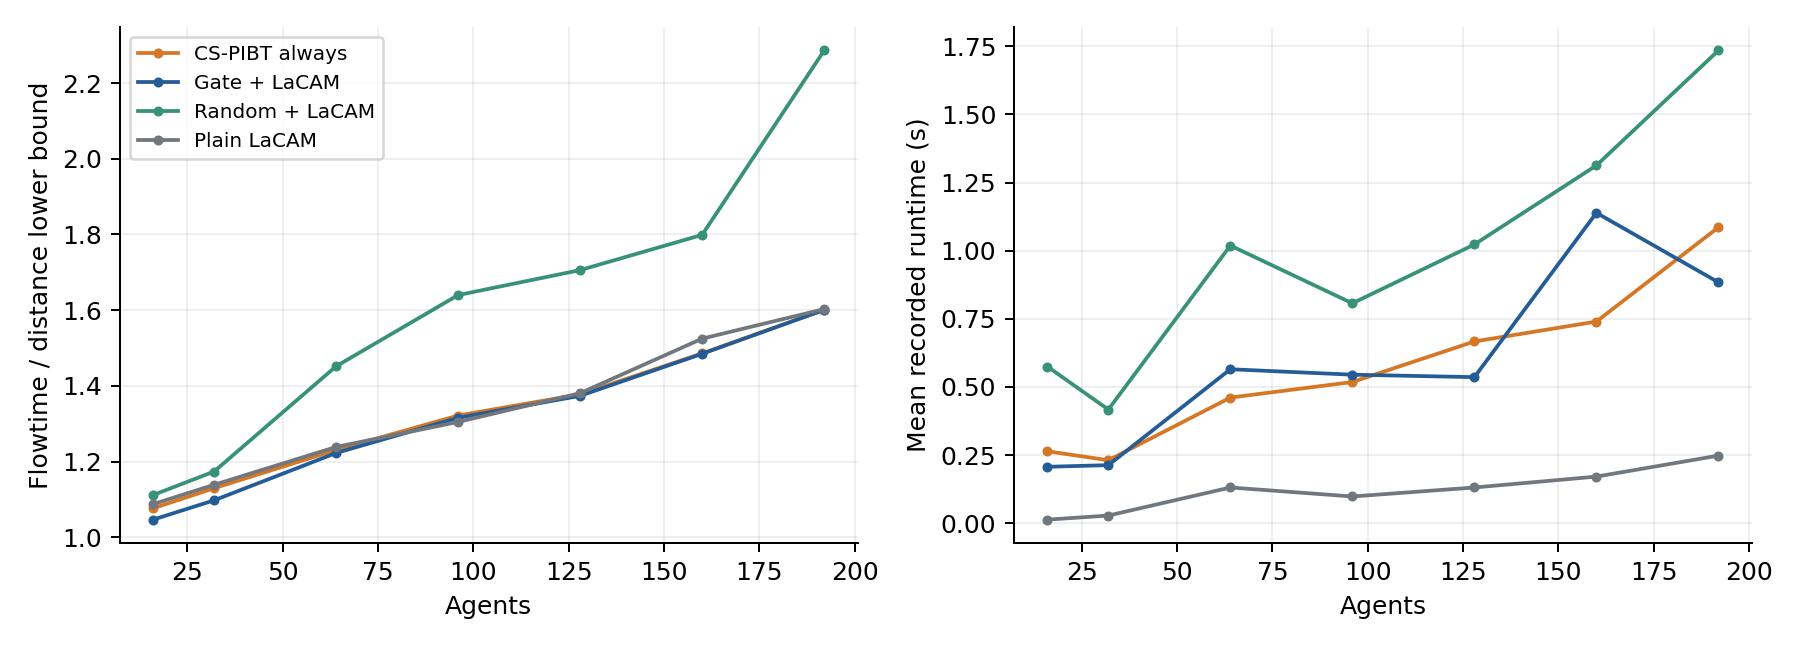
\includegraphics[width=\textwidth]{quality_runtime.png}
\caption{Common-subset solution quality and mean recorded runtime. Lower is better.}
\end{figure}
Without fallback, the selected gate threshold solves 72\% of 100 sweep instances at mean 68.7\% search frequency. Random triggering with probability 0.2 solves 88\% at realised frequency 20.3\%; probability 0.6 solves 93\% at 60.9\%. High label AUC therefore does not establish good episode reliability. Rates are not exactly equal and the learned sweep extends farther, so a random advantage at every possible compute level is not established.

A plausible interpretation is that the gate targets obvious short-term inefficiency while occasional random search disrupts persistent jams. This is not an isolated causal finding. The largest positive coefficient is conflict fraction ($+6.184$); mean maximum probability is negative ($-1.069$). Correlated coefficients do not show that confidence always increases in jams.

\newpage
\section{Demonstration and reproducibility}
The browser simulator replays actual Python trajectories and supplied models. It supports six controllers, seeded maps, playback controls and robot selection with the $11\times11$ observation window. Telemetry shows goal completion, distance remaining, gate score, external search calls, LaCAM calls/nodes and recorded time. Displayed transitions are checked for adjacency, obstacles, vertex conflicts and swaps.

The comparison table performs three fresh runs per controller after policy warm-up, displaying median time and timing range, calls, completion, flowtime and makespan, with CSV export. Repeats on one seed measure timing variation, not success across independent maps. LaCAM planning time is charged before its first plan move, and animation speed is unrelated to runtime. Demo timing includes lightweight tracing; archived main runs predate this instrumentation. Seed 42 with 64 agents illustrates shield failure and hybrid completion; seed 43 with 128 illustrates a fallback.

The code package includes implementation, demo assets, trained weights, gate/order settings, raw and summary CSVs, logs, dependencies, report source and smoke checks. From the package root:
\begin{verbatim}
python -m pip install -r requirements.txt
python -m hybrid_mapf.smoke_check
python -m hybrid_mapf.demo
python report/build_assets.py
\end{verbatim}
The asset generator verifies summaries against all 2,500 raw runs before generating evidence. The README documents full evaluation and training. Checkpoints must be moved aside in a working copy for fresh evaluation. The historical R-tuning helper removes sampling when writing its configuration; the final setting must retain both \texttt{R=0.5} and \texttt{sample=true}. Exact retraining and timing equivalence across devices are not claimed.

\section{Limitations and future work}
Plain LaCAM solves all tested maps faster, so external-call savings do not demonstrate a general speed advantage. Experiments cover one random-grid size, twenty instances per count and no standard warehouse/room/maze suite. A global gate may trigger team-wide work for one local conflict. Labels optimise eight-step progress rather than episode completion, and gate states are correlated within trajectories. Policy action validation shares maps with training; quality uses a common solved subset. Random frequency matching is retrospective and fallback budgets differ.

Future work should target episode outcomes or longer-horizon value, gate conflict groups or individual agents, and test structured maps where search is costly. Stronger evaluation would pre-calibrate random controls, equalise fallback work and measure realised time on documented hardware. Window-size and label-horizon ablations would test current choices.

\section{Conclusion}
The hybrid solves all 140 tested instances with competitive common-subset flowtime and about 23--57\% fewer external CS-PIBT invocations than always-search. However, the gate alone remains weaker than random triggering across much of the observed rate range, and plain LaCAM is faster on these maps. Predicting short-term search benefit and preventing episode failure are distinct objectives, requiring closed-loop evaluation against strong baselines.
\begingroup\small
\begin{thebibliography}{9}\setlength{\itemsep}{0pt}
\bibitem{veerapaneni} R. Veerapaneni et al. \emph{Improving Learnt Local MAPF Policies with Heuristic Search}. ICAPS, 2024. Supplied reading; extended version arXiv:2403.20300.
\bibitem{pibt} K. Okumura, M. Machida, X. D\'efago and Y. Tamura. \emph{Priority inheritance with backtracking for iterative multi-agent path finding}. Artificial Intelligence, 310:103752, 2022.
\bibitem{lacam} K. Okumura. \emph{LaCAM: Search-Based Algorithm for Quick Multi-Agent Pathfinding}. arXiv:2211.13432, 2022; cited in the supplied reading.
\bibitem{address} T. Phan, B. Zhang, S.-H. Chan and S. Koenig. \emph{Anytime Multi-Agent Path Finding with an Adaptive Delay-Based Heuristic}. AAAI, 2025. Supplied reading.
\end{thebibliography}\endgroup
\end{document}
